\documentclass[a4paper,onecolumn,10pt]{article}
\usepackage[polish]{babel}
\usepackage[utf8]{inputenc}
\usepackage[T1]{fontenc}
\usepackage[left=2.1cm,right=2.1cm]{geometry}
\usepackage[dvipsnames]{xcolor}
\usepackage{amsmath,calc,indentfirst,fancyhdr,amsfonts,graphicx,epstopdf,caption, mathcomp, subcaption,wrapfig, siunitx,pbox,float,algorithm}
\usepackage[noend]{algpseudocode}


\makeatletter
\def\BState{\State\hskip-\ALG@thistlm}
\renewcommand{\ALG@name}{Algorytm}
\makeatother

\renewcommand{\baselinestretch}{1.1}	 % odstep miedzy liniami
\addto\captionspolish{\renewcommand{\figurename}{Wykres}} % zmiana podpisu pod obrazkami, zamiast "Rysunek" bedzie "Wykres"
\newcommand{\NN}{\mathbb{N}}			 % makro do znaku liczb naturalnych

\newcommand{\R}[1]{\textcolor{red}{#1}}  % makro do polecenia z parametrami - tutaj 1 parametr
\newcommand{\G}[1]{\textcolor{green}{#1}} 
\newcommand{\B}[1]{\textcolor{RoyalBlue}{#1}} 
% kolorowanie {\B{argument}}

\newcommand{\PICTURES}{} % szybsza kompilacja dzieki stalej "usuwajacej" obrazki
						 % zakomentowanie \PICTURES powoduje znikniecie obrazkow

\pagestyle{fancy} % formatuj caly dokument
\fancyhead{}
\fancyfoot{}
\renewcommand{\headrulewidth}{0pt}
\fancyfoot[R]{\thepage} % dla stron poza tytulowa nr w prawym dolnym rogu

\fancypagestyle{plain}{ % dla strony tytulowej nr w prawym dolnym rogu
	
	\renewcommand{\headrulewidth}{0pt}
	\fancyhf{}
	\fancyfoot[R]{\thepage}
}

\renewcommand{\arraystretch}{1.2}

\title{\Large\vspace{-2.5cm}{\Huge S}PRAWOZDANIE - LABORATORIUM NR {\Huge6}\\
		\textbf{Wyznaczanie zer wielomianu metodą siecznych} } 
\date{\Large4 kwietnia 2019}
\author{\Large Marek Kiełtyka}

\begin{document}
\maketitle

\vspace{-1.2cm}\section{Wstęp}
	
\subsection{Metoda siecznych}

Jest to jedna z iteracyjnych metod numerycznych służących do wyznaczania pierwiastków równań nieliniowych. Opiera się na założeniu o ciągłości niektórych funkcji wielomianowych. Każdą taką funkcję można przybliżyć w sposób liniowy na odcinku dążącym w swej długości do zera. W miejscu przyjętego przedziału $ [x_i, x_j] $ krzywą reprezentującą przebieg funkcji zastępuje się sieczną, którą prowadzi się do momentu przecięcia jej z osią $ OX $. Kolejne coraz dokładniejsze przybliżenia dążą do ściśle określonego punktu przecięcia, który de facto jest poszukiwanym miejscem zerowym.
\subsubsection{Niemodyfikowana metoda siecznych}

Klasyczna wersja metody opiera się o zastosowanie iteracyjnego wzoru:
\begin{equation}
x_{k+1} = x_k - \frac{x_k - x_{k-1}}{f(x_k) - f(x_{k-1})}f(x_k),
\label{iter}
\end{equation}
gdzie $ k $ - numer iteracji. Konieczne jest spełnienie założenia twierdzenia Bezoute'a, które narzuca\,warunek
\begin{equation}
f(x_{k})f(x_{k-1}) < 0, 
\end{equation}
gdyż tylko wtedy sieczna przechodząca przez punkty $ (x_k, f(x_k)) $  i $ (x_{k-1},f(x_{k-1})) $ przetnie oś $ OX $. Zwykle stosuje się kryterium zbieżności, aby nie iterować w nieskończoność i szybko otrzymać niezaburzone wyniki.

\subsubsection{Modyfikowana metoda siecznych}

Odnosząc się do klasycznej metody polega ona na tym samym wzorze z jedną zasadniczą różnicą. Badaną funkcję $ f $ zastępujemy inną, która za przykładem laboratorium może powstać np. z dokonywania operacji na $ f $. W tym przypadku wykorzystano przepis:
\begin{equation}
u(x) = \frac{f(x)}{f'(x)}
\end{equation}
i wstawiono go w odpowiednie miejsce wzoru (\ref{iter}). Przy komputerowych obliczeniach numerycznych warto wykorzystać przybliżenie pochodnej funkcji ilorazem różnicowym
\begin{equation}
f'(x) = \frac{df(x)}{dx} = \frac{f(x + \Delta x) - f(x - \Delta x)}{2\Delta x}
\end{equation}
aniżeli obliczać ręcznie pochodną wielomianu wysokiego stopnia.

\newpage
\section{Zadanie do wykonania}

\subsection{Opis problemu}

Celem laboratorium było wyznaczenie pierwiastków funkcji wielomianowej 
\begin{equation}
f(x) = (x-1.2)(x-2.3)(x-3.3)^2
\label{funkcja}
\end{equation}
opisywanymi metodami: 
\begin{itemize}
	\item niemodyfikowaną dla wszystkich miejsc zerowych,
	\item modyfikowaną dla pierwiastków o krotności większej od 1 z krokiem $ \Delta x = 0.1 $ oraz $ \Delta x = 0.001 $. 
\end{itemize}
Wzór (\ref{iter}) wymaga warunków początkowych, toteż dla widocznych z postaci (\ref{funkcja}) szukanych rozwiązań założono odpowiednio
\begin{enumerate}
	\item $ x_0 = 0.9, x_1 = 1.0 $
	\item $ x_0 = 1.7, x_1 = 1.75 $
	\item $ x_0 = 3.7, x_1 = 3.65 $.
\end{enumerate}
Ponadto przyjęto warunek zbieżności na poziomie 
\begin{equation}
\epsilon_{k+1} = |x_{k+1} - x_k| < 10^{-6}.
\end{equation}


\subsection{Wyniki}

Korzystając z programu napisanego w języku C++ zaimplementowano obie metody dla wymienionych przypadków. Sporządzono wykres funkcji i jej pochodnej, a także osobne tabele w celu śledzenia postępów i czasu osiągania zbieżności. Dokonano obliczeń dla podwójnej precyzji.

\begin{table}[!hb]
	\centering
	\label{pierwsze}
	\caption{Tabele przybliżeń pierwszych dwóch miejsc zerowych wyszukiwanych \textbf{niemodyfikowaną metodą siecznych}; w kolumnach kolejno: $ k $ – numer iteracji, $ x_{k+1} $ – przybliżenie miejsca zerowego w danej iteracji, $\epsilon_{k+1}$ – różnica między dwoma ostatnimi przybliżeniami, $ f(x_{k+1}) $ – wartość funkcji w punkcie $ x_{k+1} $.}

	\begin{tabular}{|c|c|c|c|}
%		\label{pierwsze}
%		\centering
%		\caption{Pierwsze miejsce zerowe: $ x = 1.2 $ (dla $ x_0 = 0.9, x_1 = 1.0 $)}
	\hline
	k&$x_{k+1}$&$\epsilon_{k+1} $&$ f(x_{k+1})$ \\ \hline
	1&1.13177&0.131769&0.374736 \\ \hline
	2&1.18111&0.0493456&0.0948721 \\ \hline
	3&1.19784&0.0167279&0.0105107 \\ \hline
	4&1.19993&0.00208415&0.000358444 \\ \hline
	5&1.2&7.35846e-005&1.43563e-006 \\ \hline
	6&1.2&2.95904e-007&1.97418e-010 \\ \hline
	\end{tabular}
\hfill
	\begin{tabular}{|c|c|c|c|}
		\hline
%		\label{drugie}
%		\centering
%		\caption{Drugie miejsce zerowe: $ x = 2.3 $ (dla $ x_0 = 1.7, x_1 = 1.75 $)}
		k&$x_{k+1}$&$\epsilon_{k+1} $&$ f(x_{k+1})$ \\ \hline
		1&2.63105&0.88105&0.212 \\ \hline
		2&2.43208&0.198968&0.122586 \\ \hline
		3&2.1593&0.272784&-0.17563 \\ \hline
		4&2.31995&0.160652&0.0214606 \\ \hline
		5&2.30246&0.0174929&0.00269569 \\ \hline
		6&2.29994&0.00251296&-6.13175e-005 \\ \hline
		7&2.3&5.58899e-005&1.65087e-007 \\ \hline
		8&2.3&1.5007e-007&1.00372e-011 \\ \hline
	\end{tabular}
\end{table}

\begin{table}[!htp]
	\centering
	\label{pierwszetrzecie}
	\caption{Tabele przybliżeń trzeciego miejsca zerowego wyszukanego \textbf{niemodyfikowaną metodą siecznych}; w kolumnach kolejno: $ k $ – numer iteracji, $ x_{k+1} $ – przybliżenie miejsca zerowego w danej iteracji, $\epsilon_{k+1}$ – różnica między dwoma ostatnimi przybliżeniami, $ f(x_{k+1}) $ – wartość funkcji w punkcie $ x_{k+1} $.}
	\begin{tabular}{|c|c|c|c|}
		\hline
	k&$x_{k+1}$&$\epsilon_{k+1} $&$ f(x_{k+1})$ \\ \hline
	1&3.51916&0.130842&0.135802 \\ \hline
	2&3.45319&0.0659641&0.0609795 \\ \hline
	3&3.39943&0.0537603&0.0239082 \\ \hline
	4&3.36476&0.0346713&0.00966736 \\ \hline
	5&3.34123&0.0235366&0.00378918 \\ \hline
	6&3.32605&0.0151721&0.00148075 \\ \hline
	7&3.31632&0.00973224&0.000572969 \\ \hline
	8&3.31018&0.00614271&0.000220855 \\ \hline
	9&3.30633&0.00385286&8.48219e-005 \\ \hline
	10&3.30392&0.00240241&3.25142e-005 \\ \hline
	11&3.30243&0.00149333&1.24463e-005 \\ \hline
	12&3.3015&0.000926181&4.76059e-006 \\ \hline
	13&3.30093&0.00057368&1.81991e-006 \\ \hline
	14&3.30058&0.000355037&6.9551e-007 \\ \hline
	15&3.30036&0.000219611&2.65747e-007 \\ 
	\end{tabular}
	\begin{tabular}{|c|c|c|c|}
	16&3.30022&0.000135798&1.01527e-007 \\ \hline
	17&3.30014&8.39552e-005&3.87845e-008 \\ \hline
	18&3.30008&5.18976e-005&1.48155e-008 \\ \hline
	19&3.30005&3.20784e-005&5.65929e-009 \\ \hline
	20&3.30003&1.98271e-005&2.16172e-009 \\ \hline
	21&3.30002&1.22544e-005&8.25718e-010 \\ \hline
	22&3.30001&7.57385e-006&3.154e-010 \\ \hline
	23&3.30001&4.68098e-006&1.20473e-010 \\ \hline
	24&3.3&2.89304e-006&4.60167e-011 \\ \hline
	25&3.3&1.78801e-006&1.75769e-011 \\ \hline
	26&3.3&1.10505e-006&6.71378e-012 \\ \hline
	27&3.3&6.82963e-007&2.56444e-012 \\ \hline
	28&3.3&4.22095e-007&9.79529e-013 \\ \hline
%		\caption{Trzecie miejsce zerowe: $ x = 3.3 $ (dla $ x_0 = 3.7, x_1 = 3.65 $)}
%		\label{trzecie}
	\end{tabular}
%	\end{minipage}
\end{table}
\begin{table}[!htp]
	\centering
	\label{drugie}
	\caption{Tabele przybliżeń dwukrotnego miejsca zerowego $ x = 3.3 $, wyszukiwanego \textbf{modyfikowaną metodą siecznych}; w kolumnach kolejno: $ k $ – numer iteracji, $ x_{k+1} $ – przybliżenie miejsca zerowego w danej iteracji, $\epsilon_{k+1}$ – różnica między dwoma ostatnimi przybliżeniami, $ f(x_{k+1}) $ – wartość funkcji w punkcie $ x_{k+1} $. Tabele:\\\textbf{po lewej:} iloraz różnicowy obliczany z krokiem $ \Delta x = 0.1 $, \\\textbf{po prawej:} iloraz różnicowy obliczany z krokiem $ \Delta x = 0.001 $.}
	\begin{tabular}{|c|c|c|c|}
		\hline
		k&$x_{k+1}$&$\epsilon_{k+1} $&$ f(x_{k+1})$ \\ \hline
		1&3.25065&0.399349&0.0047475 \\ \hline
		2&3.32054&0.0698935&0.000913445 \\ \hline
		3&3.30675&0.0137991&9.65125e-005 \\ \hline
		4&3.30297&0.00377639&1.85962e-005 \\ \hline
		5&3.30161&0.00136042&5.44866e-006 \\ \hline
		6&3.30091&0.000694918&1.7565e-006 \\ \hline
		7&3.30054&0.00037378&6.13227e-007 \\ \hline
		8&3.30032&0.000215585&2.21348e-007 \\ \hline
		9&3.3002&0.000127248&8.17992e-008 \\ \hline
		10&3.30012&7.66162e-005&3.06083e-008 \\ \hline
		11&3.30007&4.65704e-005&1.15467e-008 \\ \hline
		12&3.30005&2.84972e-005&4.37654e-009 \\ \hline
		13&3.30003&1.75031e-005&1.6638e-009 \\ \hline
		14&3.30002&1.07765e-005&6.33659e-010 \\ \hline
		15&3.30001&6.64457e-006&2.416e-010 \\ \hline
		16&3.30001&4.10062e-006&9.21802e-011 \\ \hline
		17&3.3&2.53205e-006&3.51855e-011 \\ \hline
		18&3.3&1.56403e-006&1.34339e-011 \\ \hline
		19&3.3&9.66291e-007&5.12996e-012 \\ \hline
		20&3.3&5.97074e-007&1.95915e-012 \\ \hline
	\end{tabular}
\hfill
	\centering
	\begin{tabular}{|c|c|c|c|}
		\hline
		k&$x_{k+1}$&$\epsilon_{k+1} $&$ f(x_{k+1})$ \\ \hline
		1&3.24179&0.408215&0.00651669 \\ \hline
		2&3.31242&0.0706299&0.000329644 \\ \hline
		3&3.30056&0.0118593&6.49539e-007 \\ \hline
		4&3.3&0.000560219&3.87543e-011 \\ \hline
		5&3.3&5.18779e-006&1.67059e-012 \\ \hline
		6&3.3&4.46132e-007&4.17323e-013 \\ \hline
	\end{tabular}
\end{table}
\begin{figure}[h!]
	\begin{center}
		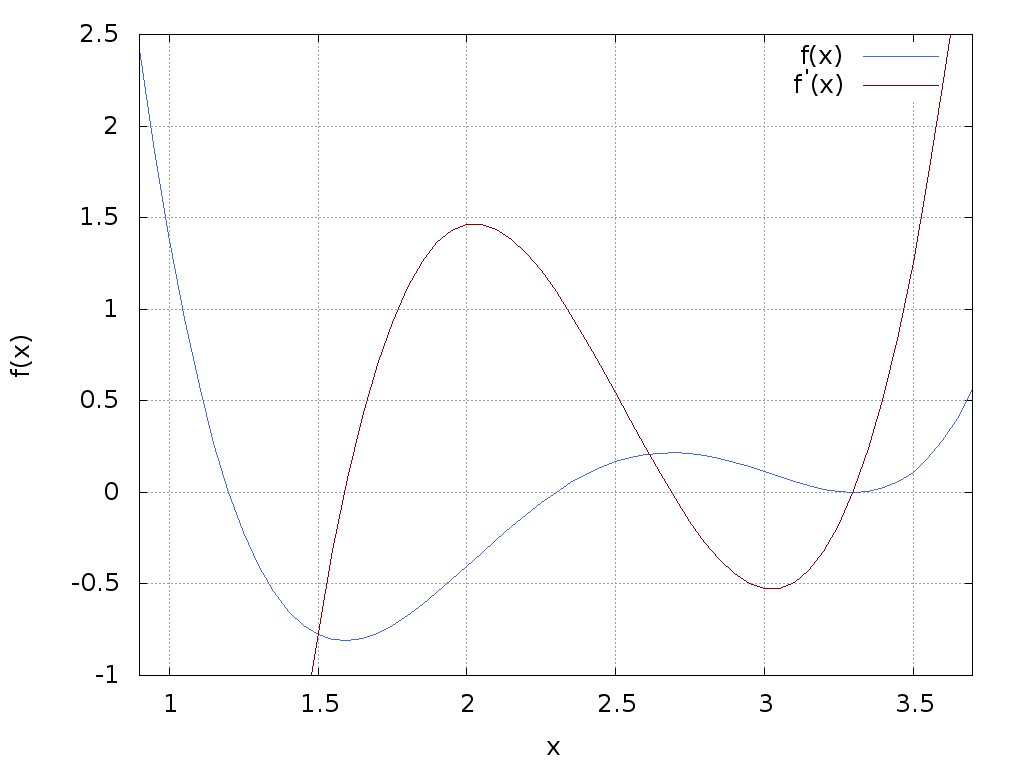
\includegraphics[height=0.4\linewidth]{funkcje.png}
		\caption{Wykres funkcji $ f(x) = (x-1.2)(x-2.3)(x-3.3)^2$ oraz jej pochodnej $ f'(x) $ w przedziale $ x \in [0.9,3.7] $}
		\label{funkcje}
	\end{center}
\end{figure}

\newpage
\section{Wnioski}

Niemodyfikowana metoda siecznych dała skuteczne rezultaty w stosunkowo krótkim okresie iterowania. Założenie progu zbieżności rzędu $ 10^{-6} $ było bardzo rozsądne, jeśli spojrzeć na wartości $ f(x_{k+1}) $ w\,każdej tabeli. Można było co prawda dalej dążyć do zera, lecz przybliżenia są na tyle satysfakcjonujące, że z oszczędności czasu wręcz należy poprzestać na takim wyniku.

Ciekawie prezentuje się modyfikacja metody. Dla niej co prawda duży krok ilorazu różnicowego nie gwarantuje znaczących usprawnień, lecz potencjał ujawnia się w momencie założenia niskiej jego wartości. Miejsca zerowe są wyznaczane ponad 3 razy szybciej, nie tracąc na dokładności.

Tabele i wykres kończą dowód na poprawność przeprowadzonych obliczeń.

\end{document}